\chapter{The H-R Diagram}

%TODO after setting "log", tell them that you can right-click and drag vert and horiz to adjust the brightness scale
%TODO  

\section{Introduction}

In this lab we will analyze our observations of star clusters taken with the Stone Edge Observatory (SEO) to make one of the key figures in all of observational astronomy - the Hertzsprung-Russell (H-R) Diagram. This will give us insight into the stellar populations in the clusters we observe, and allow us to estimate the age of their constituent stars. 

\section{Learning goals}

\begin{itemize}
    \item Gain an understanding of astronomical observation, image analysis and photometry
	\item Gain practice performing basic calculations on datasets and making informative scientific figures from those data
	\item Learn where different stellar populations lie on the HR diagram, and understand the physical reasons behind these localizations
	\item Estimate stellar cluster ages using the predictions of stellar evolutionary models. 
\end{itemize}

\textbf{Rubric rows to be assessed:} D1, D4, F1, F2, G2, G4, G5

\section{Scientific background}

Stars evolve (i.e., change their properties) over millions and often billions of years – too slow for us to see the evolution over a human lifespan.  Such impressive longevity is due to the fact that stars are powered by thermonuclear reactions, which are very efficient in generating abundant energy and have quite a bit of fuel to last for a long time. Stars like our Sun last about 10 billion years (so the Sun is in its middle age). The long timescale of evolution also means that we have to develop a different way to study stellar evolution. 

Astronomers explore evolution of stars by observing large populations of stars where different stars are in different stages of evolution. Of course, in order to do this we need to be able to tell which star is in what stage. This is done by a combination of observations – which measure luminosity and surface temperatures – and theoretical models – which predict how luminosity and surface temperature change as stars evolve. The key is that luminosity and temperature at a certain age are determined by star's mass, chemical composition, and details of thermonuclear reactions (which elements are burning, over what fraction of star's volume, etc.).

Luminosity and temperature of stars are related because they are both determined by their internal structure, which, in turn, is determined by the basic physical properties (mass, chemical composition, age). Therefore, stars are not scattered randomly in the luminosity and temperature space but follow well-defined sequences, which reflect the ranges of the controlling parameters in a given stellar population. 

The surface temperatures of stars can be deduced by fitting a blackbody radiation spectrum to their spectra. Even for stars that do not have spectra measured, their temperatures can be deduced from their colors (Recall: does bluer color correspond to cooler or hotter temperature?). Our eyes and brain perceive color by analyzing spectral composition of the incoming light. In astronomy, a star's color is defined as the difference between its magnitudes measured through two different filters that block out all light except light within a fairly narrow range of wavelengths. 

In order to interpret evolutionary states, we look at physical groupings of stars called stellar clusters, which are located at the same distance from us and were born at the same time from the same cloud of dense gas. The spread in their properties will thus not be due to different ages or initial compositions, but mainly due to different masses. As you will see, stars occupy distinct regions of the observable equivalent of the luminosity-temperature space – the magnitude-color space called the Hertzsprung-Russell (HR) diagram. We will make this diagram for the star cluster we observed.

\section{Astronomical Observation: A Brief Overview}

\subsection{Telescopes}

A \textbf{telescope} is any tool an astronomer uses to collect light from astronomical objects. Telescopes are effectively light buckets --- they enable the visualization and analysis of astronomical objects by collecting enough light that these faint sources can be detected. This is enabled by a large \textbf{primary mirror} off of which incident light is reflected and focused into an eyepiece or onto a detector. A schematic for a type of telescope similar to the Stone Edge observatory is given in Fig~\ref{telescope_schematic}. Thus the surface area of the primary mirror indicates the light-gathering abilities of a telescope: the human pupil is at most $\sim8\textrm{mm}$ in diameter, while the largest amateur telescopes have apertures approaching $\sim20\textrm{cm}$, and the largest observatories in the world have primary mirrors of up to $10\textrm{m}$. The telescope we used for these observations has a $50\textrm{cm}$ diameter, giving it the light-gathering power of approximately 3000 maximally-dilated human eyes!

\begin{figure}
\label{telescope_schematic}
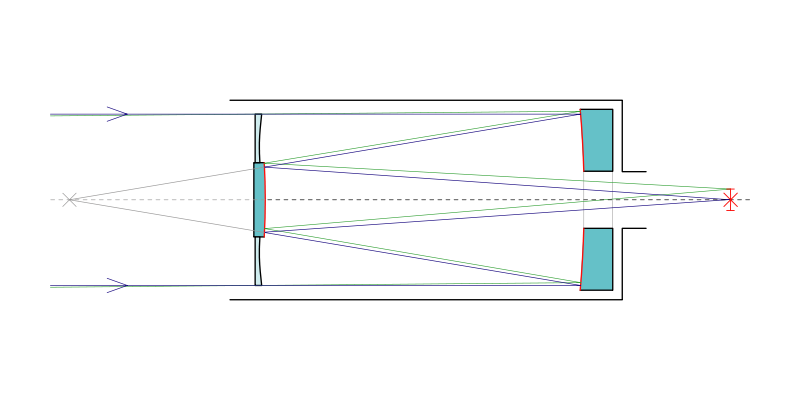
\includegraphics[scale = 0.5]{hr_diagram/Schmidt-Cassegrain-Telescope.png}
\caption{Schematic for a reflection telescope of a Schmidt-Cassegrain design, similar to the SEO telescope used to take the data for this lab.
Light rays from astronomical objects enter the telescope in parallel because their source is effectively at infinite distance. They are then reflected by a parabolic primary mirror onto a secondary mirror that again reflects the light to a focus. An eyepiece or a camera is placed at the focal plane of the resulting image. Image source: \texttt{https://en.wikipedia.org/wiki/Cassegrain\_reflector\#/media/File:Schmidt-Cassegrain-Telescope.svg}}
\end{figure}

\subsection{Filters}
Light is composed of energy-packets termed \textbf{photons} with energies that determine their wavelengths (sorter wavelength $\implies$ higher energy). Thus every light source exhibits a \textbf{spectrum} of energies based on its components, which are determined by the physics of the light emission process. Observing the spectrum of radiation emitted from astronomical objects is a fundamental tool in observational astrophysics. However, obtaining the specific intensity of radiation as a function of energy for many dim sources is challenging. An easier way to asses the electromagnetic energies observed is to image them in different \textbf{filters}: materials placed at the opening of a telescope that are transparent to a known range of wavelengths and opaque to all others (thus ``filtering'' the light). Thus, one can image the same object with multiple different filters to get a sense of the wavelength regimes that dominate the light from a source.

A filer is characterized by its \textbf{transmission function}: a function that characterizes the amount of light that is transmitted by the filter at each wavelength. Figure~\ref{sdss_filters} shows the transmission functions for some standard astronomical filters (similar to the one's you'll be using in this class).

\begin{figure}
\label{sdss_filters}
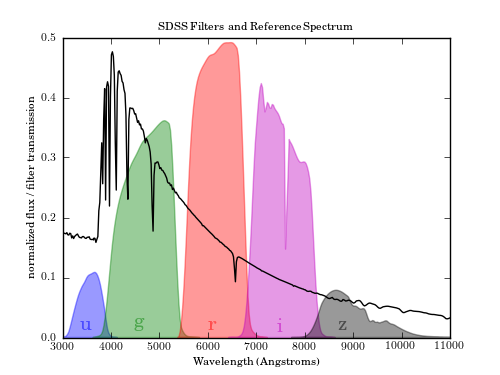
\includegraphics{hr_diagram/fig_sdss_filters_1.png}
\caption{Filter Transmission Functions for the Sloan Digetal Sky Survey, overlaid on a stellar spectrum. The magnitude observed by each filter will be proportional to the integrated spectrum multiplied by the filter transmission. It's clear in this image that the underlying spectrum of the star will cause the different filters to have different magnitudes. Image source: \texttt{http://www.astroml.org/\_images/fig\_sdss\_filters\_1.png}}
\end{figure}

\subsection{CCD Cameras}

While telescopes do the job of gathering and focusing light from astronomical objects, and filters isolate an energetic subset of that light, one needs an attached detector to record images digitally for further analysis. Modern astronomical observation primarily uses \textbf{Charge Coupled Devices (CCDs)} for this purpose. Every time a photon hits the detector, an electron is knocked off of the incident pixel, effectively charging that pixel. Thus, for each pixel, more photons $\implies$ more electrons $\implies$ more charge, and the charge can be read off into a digital signal that is then processed as an image. In this way, the brightness of the image on the detector is measured at each pixel. This brightness information constitutes the digital images astronomers analyze to understand their observational targets, as we will do in this lab. 

\section{Obtaining Observational Data}

To view images taken by the SEO and download the associated data, sign into your account on the queue website (\texttt{https://queue.stoneedgeobservatory.com/}), navigate to \texttt{OBSERVATIONS} $\blacktriangleright$ \texttt{MY OBSERVATIONS}. The observation you queued should be listed, and \texttt{Yes} should appear in the \texttt{Completed} column if the data have been taken. To view and download completed observations, click \texttt{Actions} $\blacktriangleright$ \texttt{Go To Images}. This will link you to an external page with both an image viewer and links to directly download the data. One of your observations should be immediately visible. To download your data, click \texttt{View Selected AOR Folder}, which contains the data products of your observation, and download the files that end in \texttt{BDF.fits} --- there should be one for each filter. If for some reason you lack this file for \textit{either} of your filters, ask for both from another group. You need to analyze data from both filters using the same exposure time.

%This can be accomplished with the \texttt{Download Selected FITS File}. Make sure that the \texttt{Pipe Step} option under \texttt{Selection} is listed as \texttt{FludxCalibrated}, since this is the reduced and calibrated data. There are other data products from both the observation and data reduction process available from this page, but we aren't using them for our analysis. Unfortunately, the data reduction process does not work on every observation, so if one or both of your observations lacks \texttt{FluxCalibrated} option, share data with a group that does.\textit{Note that you cannot use data from different observations for both filters - i.e. observations from both filters analyzed by each group need to be of the same exposure time}. Download these data onto your local machine where you will perform your analysis.

\section{Analyzing the data in DS9}

To analyze our observations we will be using DS9 (\texttt{http://ds9.si.edu/site/Home.html}), a popular software package for the visualization and basic analysis of image data within the astronomical community. If you are working on a lab computer, the software is already installed. If you are using your personal computer, it can be downloaded and installed from the provided link. 

We will use this tool to measure the flux in both observed filters for as many stars as possible. Each group should use separate, adjacent computers - bring up images in DS9 for each filter, one filter per computer. To better visualize the images in DS9, logarithmically scale the display by selecting \texttt{scale} $\blacktriangleright$ \texttt{log}. Contrast and bias of the display image can be modified by right clicking and dragging - you should adjust these so that the stars are optimally visible.

To determine how much flux comes form each star, we will use the ``regions'' functionality of DS9 that gives information about a selected region in the image. First click \texttt{edit} $\blacktriangleright$ \texttt{region}, and then you will create a region -- indicated by a green circle -- each time you click on the image. Clicking in the center of the region will allow you to move it about the image, while clicking on the edge allows you to adjust it's size. For each star you measure, you'll want to create a region that contains as much flux as possible without contamination from a nearby star or the background. Once this is accomplished, double click the region (which will cause a window with basic information to appear), and select \texttt{Analysis} $\blacktriangleright$ \texttt{Statistics}, which will cause a separate panel to appear with information about the data contained in that region. \texttt{Sum} is an instrument-and-observation specific measure of the flux --- the energy per unit surface area per unit time --- incident on the detector from the light of the astronomical object we observe. Record this value and it's listed error. How are these values related (hint: you can directly calculate the error from the sum with a simple mathematical operation)? Why are they related in this way?
% the flux (in an astronomy-specific unit called ``Janskys", abbreviated as Jy) value you should record. Also recod the ``Center" coordinates and radius of the region. Do this in both filters, for each star that you measure. \textit{Note that the error listed under ``Statistics" is \textbf{not} a correct estimate of the error in the flux value, so do not record this}.

%Error in your measurement can be the result of several causes, but one that is easy to quantify is the presence of background noise (from e.g. sky brightness or scattered light in the telescope). 

Note that even regions in the image that do not contain a discernable source have non-zero flux. This \textbf{background} is from scattered light from the earth's atmosphere (particularly when it's cloudy) and from light scattered by the apparatus inside the telescope. Since this background is not the signal we wish to analyze from our source, we should subtract it from the measured flux from each star. From several circular regions over nothing in particular, determine how many counts there are per unit area, just from the backgrounds.  The \texttt{surf$\_$bri} value gives what we need.  Do this several times to determine the variance in the background.  Thus quantify this background and its error. For each of your stars, compute the background that was likely in the aperture.  This involves multiplying the surface brightness by the area you chose.  Note that the error in the surface brightness propagates, so if you have a very big region, that will likely determine the error on your final measurement. 

Try to measure fluxes and errors for as many stars as possible in your lab session. There will inevitably be some overlap between groups, which is fine, but try to obtain measurements for stars at a wide range of brightness’s. 50 stars is a good target, but the more the better. Thirty minutes before lab ends, stop collecting data, and share your data among your section so that you can finish the rest of the analysis.

\section{Calculating Magnitudes}

In astronomy we deal with magnitudes, which are scaled logarithmically, and increase with decreasing source brightness. Specifically, the equation for the magnitude $m_X$ of an object in a wavelength band $X$ with flux $F_X$ is given by 

\begin{equation}
m_{X} = -2.5\log_{10}\left(\frac{F_X}{F_{X,{\textrm{ref}}}}\right)
\end{equation}

where $F_{X,{\textrm{ref}}}$ is a reference flux value for the given band and magnitude system. Note that the \texttt{sum} value we recorded is not actually the physical flux -- the process of converting observed image brightness's to physical fluxes is a non-trivial calibration procedure we will not undertake here. Instead, we will calculate instrument-specific magnitudes by adopting the counts from the brightest star as the reference flux $F_{X,\textrm{ref}}$. \textit{Note: you must use the same star in both bands for these magnitudes to be compared. Determine the reference star in your section, and calculate magnitudes in both bands from all of the stars measured by your section using Excel or any other software/coding language of your choice.}

%For the SDSS magnitude system we are using, $F_{\textrm{ref}} = 3631 {\textrm{Jy}}$ for both $g'$ and $r'$ measurements. Calculate magnitudes in both bands for all of the stars measured in your section. You can use Excel or any other software/coding language of your choice to do this.  

\section{Making an HR Diagram}

Since different bands measure brightness in different wavelengths, the ratio of flux in two bands is a measure of an object's color. Therefore, the difference between astronomical magnitudes of an object in different bands is a measure of its color, since the magnitude scale is logarithmic:

\begin{equation}
m_A - m_B = -2.5\log\left(\frac{F_A}{F_B}\right).
\end{equation}

An H-R diagram is a plot of stellar magnitude vs. color - aka a ``color magnitude diagram''. A star's color is an observational indication of it's surface temperature. Since all of the stars in a star cluster are at approximately the same distance, their apparent magnitude gives a good relative indicator of luminosity. Therefore, a color-magnitude diagram of stars at roughly constant distance is effectively a temperature-luminosity diagram, and stars fall in characteristic regions of this parameter space based on their mass, age, and metallicity.

We have data in two wavelength bands, so we can subtract those magnitudes to get a color measure. With the software or coding language of your choice, plot $r'$ on the y-axis and $g' - r'$ on the x-axis. Add error bars to your plot. If doing so for each data point becomes crowded on your figure, you can estimate a typical error from your data and include it in a legend. 

\section{Making an HR Diagram -- with proper photometry}

In reality, your estimated error from the background is a lower limit, since there are many other possible sources of imprecision and inaccuracy in this measurement. Moreover, our analysis was an extremely crude approximation of the photometry done by professional astronomers. Finally, you may simply have recorded values for too few stars to make a color-magnitude plot to fully populate the different regions of the color-magnitude plot --- in practice, astronomers use more automated techniques that allow them to analyze all stars in the image with adequate data. To make H-R diagrams that can be interpreted scientifically, use the data provided for the cluster you observed, each of which has a file on the course website containing data on these clusters obtained from publications in the astronomical literate (\cite{An2008} for M15, \cite{Slesnick2002} for NGC 869). Note that, if you observed NGC 869, the publicly available data was made with different filters than our observations, and thus the expected positions and shapes of stellar populations on a color-magnitude diagram change, but the same general features should be apparent. Label the different stages of stellar evolution on both the professionally reduced data and, if possible, on the data you obtained in lab.   

\section{Comparing to stellar evolution models}

The last portion of this lab involves estimating the age of these stellar populations by comparing their color magnitude diagrams with predictions from a stellar evolution model. Stellar physics is sufficiently well-understood that accurate evolutionary models have been constructed to calculate the observable properties of stars across their lifetimes. Because stars evolve in their position on the HR diagram, we can estimate the age of our observed cluster by comparing these models to our observations.

Several files containing model predictions for the magnitudes of stars at different ages (from \texttt{http://stev.oapd.inaf.it/cgi-bin/cmd}), where you can easily access the predictions of stellar evolution models with parameters you specify) are contained in files on the course website. These have been calculated using the observed metallicity of the star cluster to predict the positions of stars at ages $10^7$, $10^8$, $10^9$, and $10^{10}$ years. These are called isochrones - stellar properties as a function of stellar mass for a fixed age (and metallicity). Note that these magnitudes were calculated using prior knowledge of the star cluster metallicity, and have been corrected for cluster distance and extinction due to intervening galactic dust (taken from \cite{DurrellHarris1993} for M15 and \cite{Currie2010} for NGC 869).

Plot these isochrones on your H-R diagrams and compare them to your data to estimate the cluster age. Be sure to estimate an error on this value and explain your method in your lab report. What changes in stellar properties are represented by the different locations of isochrones of different ages? What physical processes occuring inside the star underlie those changes?


